\documentclass{article}
\usepackage{amssymb, amsmath, amsthm}
\usepackage[margin=1in]{geometry}
\usepackage{verbatim}
\usepackage{graphicx}
\usepackage{hyperref} % \url \href
\usepackage{docmute}

\usepackage{tikz}
\usetikzlibrary{shapes.geometric, arrows}
\tikzstyle{startstop} = [rectangle, rounded corners, minimum width=2cm,text centered, draw=black]
\tikzstyle{process} = [rectangle, minimum width=2cm, text centered, draw=black]
\tikzstyle{decision} = [diamond, minimum width=2cm, text centered, draw=black]
\tikzstyle{arrow} = [thick,->,>=stealth]

\newtheorem{definition}{Definition}
\newtheorem{theorem}{Theorem}
\DeclareMathOperator{\spn}{Span}


\usepackage[style=chem-acs ,backend=bibtex, sorting=none]{biblatex}
\addbibresource{autoTB.bib}

\begin{document}

\section{Character table for site symmetry groups}

To use symmetry information in the construction of a tight-binding model, we first need to 
find the concrete symmetry group and it's representations. 
In this section, our implementation to find the site symmetry group in crystal, as well as 
its subgroups and characters are described in details.

\subsection{Basic Definition}

For a point $\mathbf{x}$ in a crystal, the subgroup of the space group $G$ that leave $\mathbf{x}$
fixed is called the \emph{site symmetry groups}, which we denote $S_{\mathbf{x}}$. A space group
operation in crystal can be denoted using matrix--column pair $(\mathbf{W},\mathbf{w})$ in a chosen 
basis. Then it is straightforwardly to see that group elements in the site symmetry group only 
contain rotation part. 

Given a rotation matrix $\mathbf{W}$ belonging to a site symmetry group, it can be classified into different
types, each designated by their Hermann--Mauguin (HM) symbols, depending on its trace and determinant. 
The trace $\text{tr}\mathbf{W}$ give information of the rotation angle and determinant indicates whether 
the operation is first or second kind. 
Since trace is invariant under permutation of matrices, it does not depend on any change of basis. 
They are listed in Table \ref{T:operation_properties}. 

\begin{table}[h!]
    \centering
    \caption{Site symmetry types}
    \begin{tabular}{|c|cccccccccc|}
        \hline
        $\det$      & +1 & +1 & +1 & +1 & +1 & -1 & -1 & -1 & -1 & -1 \\ 
        $\text{tr}$ &  3 &  2 &  1 &  0 & -1 & -3 & -2 & -1 &  0 &  1 \\  
        \hline
        type        &  1 &  6 &  4 &  3 &  2 & -1 & -6 & -4 & -3 & -2 = m \\ 
        \hline
    \end{tabular}
    \label{T:operation_properties}
\end{table}

There are in total 32 crystallographic point group types so that the number of distinct site symmetry group types are
also limited to 32. They can be easily identified by counting the types of operation in the group. 
Reference table can be found in Togo and Tanaka\cite{togo_spglib_2018}.

For point groups, its group operation can be uniquely denoted using \emph{Seitz symbols}. The Seitz symbol consists of 
three parts: 1) HM symbol of the operation, 2) its characteristic direction denoted by $[uvw]$ and 3) the sense of rotation $+$ or $-$. 
The sense of rotation indicate whether the rotation is clockwise or anti-clockwise and is used for $4$, $-4$, $3$, $-3$, $6$, $-6$ only.
The characteristic direction (lattice direction) is usually given with respect to different lattice systems. We use hexagonal lattice 
for both hexagonal and rhombohedral lattice. The basis for each lattice can be found in Section 2.2 of \emph{ITA}. 

\subsection{Finding the Seitz symbol from Operation Matrix}
Given an input structure and a point $\mathbf{x}$, it is often easier to find the set of matrices that belong to the site symmetry group
$S_{\mathbf{x}}$ by trying out possible point group operations, without knowing the symmetry group or even the space group\cite{togo_spglib_2018}. 
After obtaining the complete group operations, the point group can be assigned. However, at this point, the characters of each operation is
not known and it is necessary to correctly assign their characters refering to point group character table, such as the one hosted on 
Bilbao\footnote{\url{https://www.cryst.ehu.es/rep/point.html}}. 

Although the matrix for each group operation is also specified on Bilbao database, we note that they can not be compared directly with the 
set of matrices found by calculation because of different basis used, especially for the case of site symmetry. For example, in a cubic lattice 
we may have four distinct site symmetry group of $3$ (three fold rotation) with different orientation. All of them have different 
group operations but belong to the same type of point groups. The important point here is that a suitable basis need to be established for 
the computed site symmetry group before we compare each operation with the ones given on the Bilbao database. Here, we describe the procedure
to assign standard Seitz symbol to a group of site symmetry operation matrices. Given a set of operation matrices, if we can assign for 
each operation a Seitz symbol corresponding to the Bilbao data, then the assignment of character will be straightforward.

Our algorithm for the assignment take only a set of operation matrices in cartesian coordinate as input. 
It's workflow is shown in Figure \ref{F:workflow}. 
First, the type of operation can be assigned for each operation using determinant and trace. After all operation are determined, the 
point group type can be found. 

\begin{figure}[h]
    \centering
    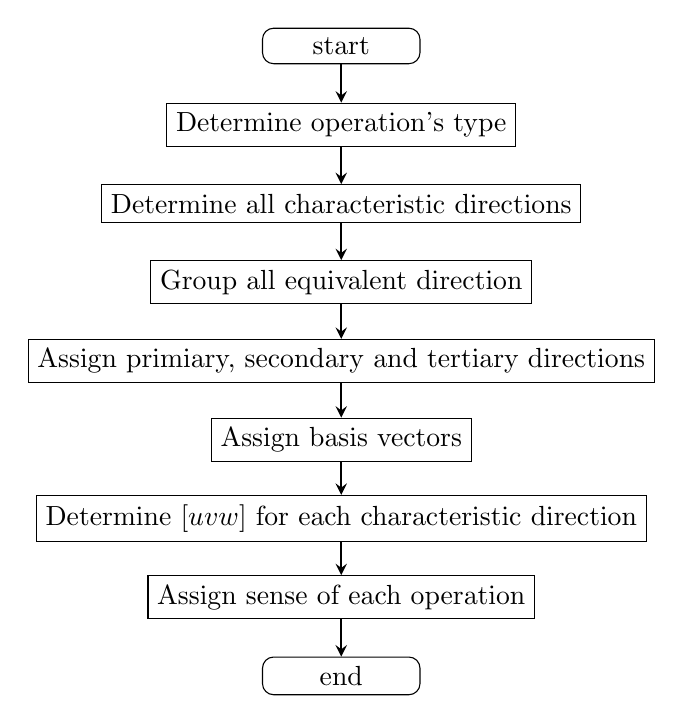
\begin{tikzpicture}[node distance=1.0cm]
        \node (start) [startstop] {start};
        \node (pro1) [process, below of=start] {Determine operation's type};
        \draw [arrow] (start) -- (pro1);
        \node (pro2) [process, below of=pro1] {Determine all characteristic directions};
        \draw [arrow] (pro1) -- (pro2);
        \node (pro3) [process, below of=pro2] {Group all equivalent direction};
        \draw [arrow] (pro2) -- (pro3);
        \node (pro4) [process, below of=pro3] {Assign primiary, secondary and tertiary directions};
        \draw [arrow] (pro3) -- (pro4);
        \node (pro5) [process, below of=pro4] {Assign basis vectors};
        \draw [arrow] (pro4) -- (pro5);
        \node (pro6) [process, below of=pro5] {Determine $[uvw]$ for each characteristic direction};
        \draw [arrow] (pro5) -- (pro6);
        \node (pro7) [process, below of=pro6] {Assign sense of each operation};
        \draw [arrow] (pro6) -- (pro7);
        \node (end) [startstop, below of=pro7] {end};
        \draw [arrow] (pro7) -- (end);
    \end{tikzpicture}
    \caption{Workflow of Seitz symbol assignment}
    \label{F:workflow}
\end{figure}

Characteristic directions can be found by finding the eigenvectors with eigenvalue of $1$. For each operation,
we first find its rotation part $\mathbf{R}$ (i.e. multiple $-\mathbf{I}$ for rotoinversion). Then, the characteristic 
direction is given by:
\begin{equation}
    \label{E:eigendirection}
    \mathbf{R}\mathbf{v} = \mathbf{v}
\end{equation}
For identity and inversion, we assigne $(0.0, 0.0, 0.0)$ as its characteristic direction. 
After computing the directions of all the symmetry operation, we separate them into groups of equivalent directions 
that are related by symmetry operations:
\begin{equation}
    \{\mathbf{v}' \mid \mathbf{W}\mathbf{v}, \mathbf{W} \in \mathbf{S_\mathbf{x}}\}
\end{equation}

These groups of equivalent symmetry directions correspond to the symmetry directions used in the Hermann-Mauguin symbol,
and knowing the symmetry operation on each direction, it is straightforward to identify the primiary, 
secondary and tertiary directions. For example, the result of an assignment at this step for group $6/mmm$
is given in Table \ref{T:6mmm}

\begin{table}[h]
    \centering
    \caption{Symmetry operation and directions in cartesian coordinate in $6/mmm$}
    \begin{tabular}{|c|l|l|}
        \hline
        Operation & Directions & Symmetry Direction\\
        \hline
        -1,1 & (  0.0  0.0  0.0) & $\mathbf{0}$\\
        6,-3,-6,m,2,3 & (  0.0  0.0  1.0) & $[001]$\\
        m,2 & (-0.5,-0.866,0.0), (1.0,0.0,0.0), (-0.5,0.866,0.0) & $[100],[010],[\bar{1}\bar{1}0]$\\
        m,2 & (0.866,-0.5,0.0), (0.0,1.0,0.0), (-0.866,-0.5,0.0) & $[120],[\bar{2}\bar{1}0],[1\bar{1}0]$\\
        \hline
    \end{tabular}
    \label{T:6mmm}
\end{table}

Then, it is possible to choose the basis for the site symmetry group. The choice of 
the basis for each group are listed in table \ref{T:choice_of_axes}. 
After choosing $\mathbf{a}$ and $\mathbf{b}$, $\mathbf{c}$ is chosen so that the three axes
form a right-handed system: $(\mathbf{a}\times \mathbf{b}) \cdot \mathbf{c} > 0$. 
Given the chosen basis, each symmetry direction as vector in cartesian coordinates, found in Equation \eqref{E:eigendirection}
can be converted to $[uvw]$ notation. Finally, the sense of rotation can be computed using $\sin\theta$ of the 
rotation angle\cite{liang_ecient_2018}.

\begin{table}[h]
    \centering
    \caption{Choice of basis for each point groups}
    \begin{tabular}{|c|c|}
        \hline
        Groups & Choice\\
        \hline
        \begin{tabular}{c}$2$, $m$, $2/m$, $4$, $-4$, $4/m$\\$3$, $-3$, $6$, $-6$, $6/m$\end{tabular}
            & $z = [001]$ \\ \hline
        $222$, $mm2$, $mmm$ & $x=[100],y=[010],z=[001]$ \\\hline
        $32$, $3m$, $-3m$, $622$, $6mm$, $-6m2$, $6/mmm$ & $\{x, y\} \in \{[100], [010],[\bar{1}\bar{1}0]\}$ \\\hline
        $23$, $m-3$, $432$, $-43m$, $m-3m$ & $\{x,y,z\} = \{[100],[010],[001]\}$ \\
        \hline
    \end{tabular}
    \label{T:choice_of_axes}
\end{table}

In our implementation, the characters associated with each point group operation are taken from the Bilbao database, and 
they are listed using the Seitz symbol. Therefore, after finding the corresponding Seitz symbol, assignment of characters to 
each operation matrix is straightforward.


\subsection{Character assignment for subgroups}

In our application, we may need to find the subgroup of the site symmetry group. 
To do so, we need to know which symmetry is kept when we move from a group to its subgroup. 

It is non-trivial to find subgroups from a set of group operation matrices directly. However, since we 
already assigned the Seitz symbol for each operation in the parent group, we can manually define a 
map between the Seitz symbol of the parent group and all its subgroups. Therefore, we only need 
to perform a simple lookup to obtain the operation and their characters for any subgroup of the site symmetry group. 
For example, a lookup table for subgroup $3$ from a parent group $432$ is given in Table \ref{T:subgrouplookup}

\begin{table}[h]
    \centering
    \caption{Defined lookup table for subgroup $3$ from $432$}
    \begin{tabular}{|c|c|}
        \hline
        Seitz symbol in $3$ & Seitz symbol in $432$\\
        \hline
        1 & 1 \\
        $3^{+}_{001}$ & $3^{+}_{111}$ \\
        $3^{-}_{001}$ & $3^{-}_{111}$ \\
        \hline
    \end{tabular}
    \label{T:subgrouplookup}
\end{table}

\subsection{Subduction}
Subduction enable us to perform symmetry descend that split the irreducible representation 
in the parent group into different irreducible representations\cite{johansson_automatic_2017}. 

For the effective split of irreducible representation of more than one dimension into distinct 
irreducible representation of the subgroup, the choice of the subgroup, i.e., which operation 
to keep as subgroup operation, is important. In our implementation, we select the subgroup operations
following the subduction table provided in \cite{altmann_point-group_1994}. 

\end{document}
